\documentclass[t,aspectratio=169]{beamer}
%\usepackage{fale}

%%% presentation below

\title{Fedora Project}
\subtitle{From a community to an Operating System}
\author{Fabio Alessandro Locati}
\date{27 October 2016}

\begin{document}

\maketitle

\begin{frame}
    \frametitle{Outline}
    \tableofcontents
\end{frame}

\section{Intro}
\begin{frame}
    \frametitle{About me} 
    \begin{itemize}
        \item<2-> Linux user since 2001
        \item<3-> IT Consultant since 2004
        \item<4-> Fedora contributor since 2013 
        \begin{itemize}
            \item<5-> Ambassador
            \item<5-> Infrastructure administrator
            \item<5-> Packager
            \item<5-> Pacakging Sponsor
        \end{itemize}
    \end{itemize}
\end{frame}

\section{Fedora Project}
\begin{frame}
    \frametitle{What is Fedora Project?}
    \begin{itemize}
        \item<2-> The Fedora Project is a partnership of Free software community members from around the globe.
        \item<3-> The Fedora Project builds open source software communities and produces a Linux distribution called "Fedora".
    \end{itemize}
    \begin{block}<4->{Mission}
        The Fedora Project's mission is to lead the advancement of Free and open source software and content as a collaborative community.
    \end{block}
\end{frame}

\section{Fedora}
\begin{frame}
    \frametitle{What is Fedora?}
    \begin{itemize}
        \item<2-> A GNU/Linux distribution
        \item<3-> 100\% FLOSS
        \item<4-> Innovating
        \item<5-> Stable
        \item<6-> Secure
        \item<7-> Easy to manage
    \end{itemize}
\end{frame}

\begin{frame}
    \frametitle{Fedora Foundations}
    \begin{center}
        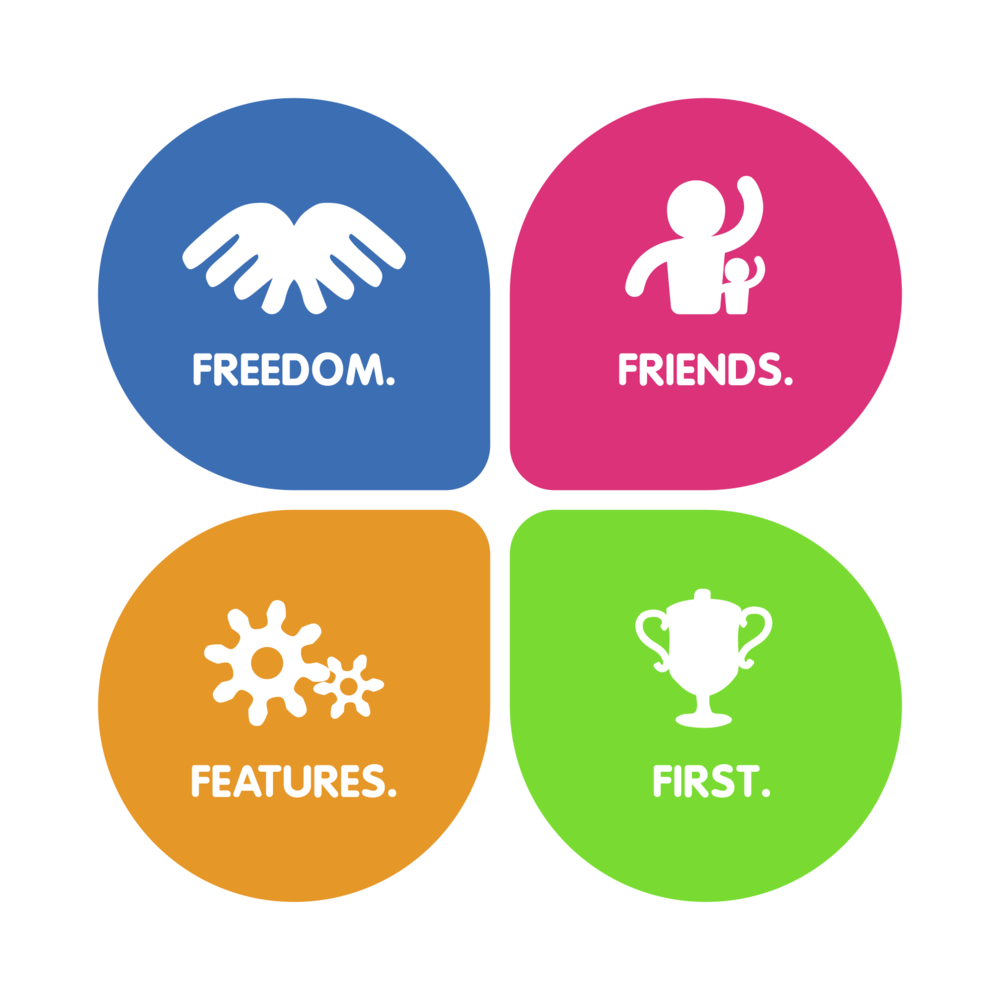
\includegraphics[scale=4.5]{foundations_all.png}
    \end{center}
\end{frame}

\begin{frame}
    \frametitle{Fedora Foundations - Freedom}
    \begin{columns}[T] % align columns
        \begin{column}{.5\textwidth}
            
\includegraphics[width=\linewidth]{foundations_expand_1_freedom.png}
        \end{column}
        \begin{column}{.5\textwidth}
            \begin{itemize}
                \item<2-> Free (as speech)
                \item<3-> Free (as beer)
                \item<4-> Legally usable for any scope
                \item<5-> Legally redistributable
                \item<6-> Legally changeable
            \end{itemize}
        \end{column}
    \end{columns}
\end{frame}

\begin{frame}
    \frametitle{Fedora Foundations - Friends}
    \begin{columns}[T] % align columns
        \begin{column}{.5\textwidth}
            
\includegraphics[width=\linewidth]{foundations_expand_2_friends.png}
        \end{column}
        \begin{column}{.5\textwidth}
            \begin{itemize}
                \item<2-> The community is the strenght of Fedora
                \item<3-> Easy to join: www.whatcanidoforfedora.org
                \item<4-> More than 5 thousands active contributors
                \item<5-> More than 13 millions users
            \end{itemize}
        \end{column}
    \end{columns}
\end{frame}

\begin{frame}
    \frametitle{Fedora Foundations - Features}
    \begin{columns}[T] % align columns
        \begin{column}{.5\textwidth}
            
\includegraphics[width=\linewidth]{foundations_expand_3_features.png}
        \end{column}
        \begin{column}{.5\textwidth}
            \begin{itemize}
                \item<2-> Commitment to excellence
                \item<3-> Many Linux innovations comes from the Fedora Community
                \item<4-> Working closely with upstream
            \end{itemize}
        \end{column}
    \end{columns}
\end{frame}

\begin{frame}
    \frametitle{Fedora Foundations - First}
    \begin{columns}[T] % align columns
        \begin{column}{.5\textwidth}
            
\includegraphics[width=\linewidth]{foundations_expand_4_first.png}
        \end{column}
        \begin{column}{.5\textwidth}
            \begin{itemize}
                \item<2-> Always aiming to the last versions of applications
                \item<3-> Historically first to embrace big changes
                \begin{itemize}
                    \item<4-> Pulseaudio by default in Fedora 8 (2007)
                    \item<5-> Systemd by default in Fedora 15 (2011)
                    \item<6-> Wayland by default in Fedora 25 (2016)
                \end{itemize}
            \end{itemize}
        \end{column}
    \end{columns}
\end{frame}

\begin{frame}
    \frametitle{Editions}
    \begin{itemize}
        \item<2-> Cloud
        \item<3-> Server
        \item<4-> Workstation
    \end{itemize}
\end{frame}

\begin{frame}
    \frametitle{Architectures}
    \begin{itemize}
        \item<2-> Primary
        \begin{itemize}
            \item<3-> ARMv7+
            \item<4-> x86
            \item<5-> x86\_64
        \end{itemize}
        \item<6-> Secondary
        \begin{itemize}
            \item<6-> AArch64 (will be upgraded in F26)
            \item<6-> MIPS64-el
            \item<6-> MIPS-el
            \item<6-> Power64 (will be upgraded in F27)
            \item<6-> Power64le
            \item<6-> RISC-V
            \item<6-> s390x (will be upgraded in F27)
        \end{itemize}
    \end{itemize}
\end{frame}

\begin{frame}
    \frametitle{Spins}
    \begin{itemize}
        \item KDE Plasma
        \item XFCE
        \item LXDE
        \item Mate and Compiz
        \item Cinnamon
        \item SOAS (Sugar)
    \end{itemize}
\end{frame}

\begin{frame}
    \frametitle{Labs}
    \begin{itemize}
        \item Astronomy
        \item Design Suite
        \item Games
        \item Robotics Suite
        \item Scientific
        \item Security lab
    \end{itemize}
\end{frame}

\begin{frame}
    \frametitle{Resources}
    \begin{itemize}
        \item Slides: https://slides.fale.io/20161027-en-fedora.pdf
        \item Fedora Project: https://fedoraproject.org
        \item Download Fedora: https://getfedora.org
    \end{itemize}
\end{frame}

%\makethanks

\end{document}
